\documentclass[11pt]{article}
\usepackage{amsmath,amsbsy,amssymb,verbatim,fullpage,ifthen,graphicx,bm,amsfonts,amsthm,url,float}
\usepackage{graphicx}
\usepackage{xcolor}
\newcommand{\mfile}[1]  {{\small \verbatiminput{./#1}}} % Jeff Fessler, input matlab file
\newcommand{\tmop}[1]{\ensuremath{\operatorname{#1}}}
%\newcommand*{\qed}{\hfill\ensuremath{\blacksquare}}%
\newcommand{\R}{\mathbb{R}}
\newcommand{\C}{\mathbb{C}}
\newcommand{\Z}{\mathbb{Z}}
\newcommand{\A}{\mathcal{A}}
\newcommand{\minimize}{\operatorname*{minimize\ }}
\newcommand{\maximize}{\operatorname*{maximize}}
\newcommand{\opdet}[1]{\operatorname{\textbf{det}}\left(#1\right)}
\newcommand{\optr}[1]{\operatorname{\textbf{tr}}\left(#1\right)}
%\newcommand{\AnswerDefine}{}
\newcommand{\answer}[2][blue]{\ifdefined\AnswerDefine{\color{#1}\it#2}\fi}
\newcommand{\mtx}[1]{\mathbf{#1}}
\newcommand{\vct}[1]{\mathbf{#1}}
\def \lg       {\langle}
\def \rg       {\rangle}
\def \mA {\mtx{A}}
\def \mF {\mtx{F}}
\def \mG {\mtx{G}}
\def \mI {\mtx{I}}
\def \mJ {\mtx{J}}
\def \mU {\mtx{U}}
\def \mS {\mtx{S}}
\def \mV {\mtx{V}}
\def \mW {\mtx{W}}
\def \mLambda {\mtx{\Lambda}}
\def \mSigma {\mtx{\Sigma}}
\def \mX {\mtx{X}}
\def \mY {\mtx{Y}}
\def \mZ {\mtx{Z}}
\def \zero     {\mathbf{0}}
\def \vzero    {\vct{0}}
\def \vone    {\vct{1}}
\def \va {\vct{a}}
\def \vg {\vct{g}}
\def \vu {\vct{u}}
\def \vv {\vct{v}}
\def \vx {\vct{x}}
\def \vy {\vct{y}}
\def \vz {\vct{z}}
\def \vs {\vct{s}}
\def \vphi {\vct{\phi}}
\def \vmu {\vct{\mu}}
\def \R {\mathbb{R}}
\def \vw {\vct{w}}

%\newcommand{\st}{\operatorname*{\ subject\ to\ }}
\usepackage{algorithm,algpseudocode}
\usepackage{xspace}
% Add a period to the end of an abbreviation unless there's one
% already, then \xspace.
\makeatletter
\DeclareRobustCommand\onedot{\futurelet\@let@token\@onedot}
\def\@onedot{\ifx\@let@token.\else.\null\fi\xspace}

\def\eg{\emph{e.g}\onedot} \def\Eg{\emph{E.g}\onedot}
\def\ie{\emph{i.e}\onedot} \def\Ie{\emph{I.e}\onedot}
\def\cf{\emph{c.f}\onedot} \def\Cf{\emph{C.f}\onedot}
\def\etc{\emph{etc}\onedot} \def\vs{\emph{vs}\onedot}
\def\wrt{w.r.t\onedot} \def\dof{d.o.f\onedot}
\def\etal{\emph{et al}\onedot} \def\st{\emph{s.t}\onedot}
\pagestyle{plain}

\title{{\bf Homework Set 3, CPSC 8420, Spring 2022}} % Change to the appropriate homework number
\author{\Large\underline{Huang, Gangtong}}
\date{\textbf{\Large\textcolor{red}{Due 03/31/2022, Thursday, 11:59PM EST}}} % put your name in the LastName, FirstName format
%\date{\today}

\begin{document}
\maketitle

\section*{Problem 1}
Given data-points $\{\{1,3\},\{2,5\},\{3,4\},\{4,3\},\{5,2\},\{5,1\}\}$.
\begin{enumerate}
	\item Please scatter-plot each data point within one figure (you can use Matlab, Python or any other programming language).\\ \\
	The scatter plot of the original data points in Fig. 1 is made with Mathematica. For the convenience of PCA, the data points centered at origin are also plotted in Fig. 1.2.
	\begin{figure}[H] % This is how figure are placed into latex document
		\centering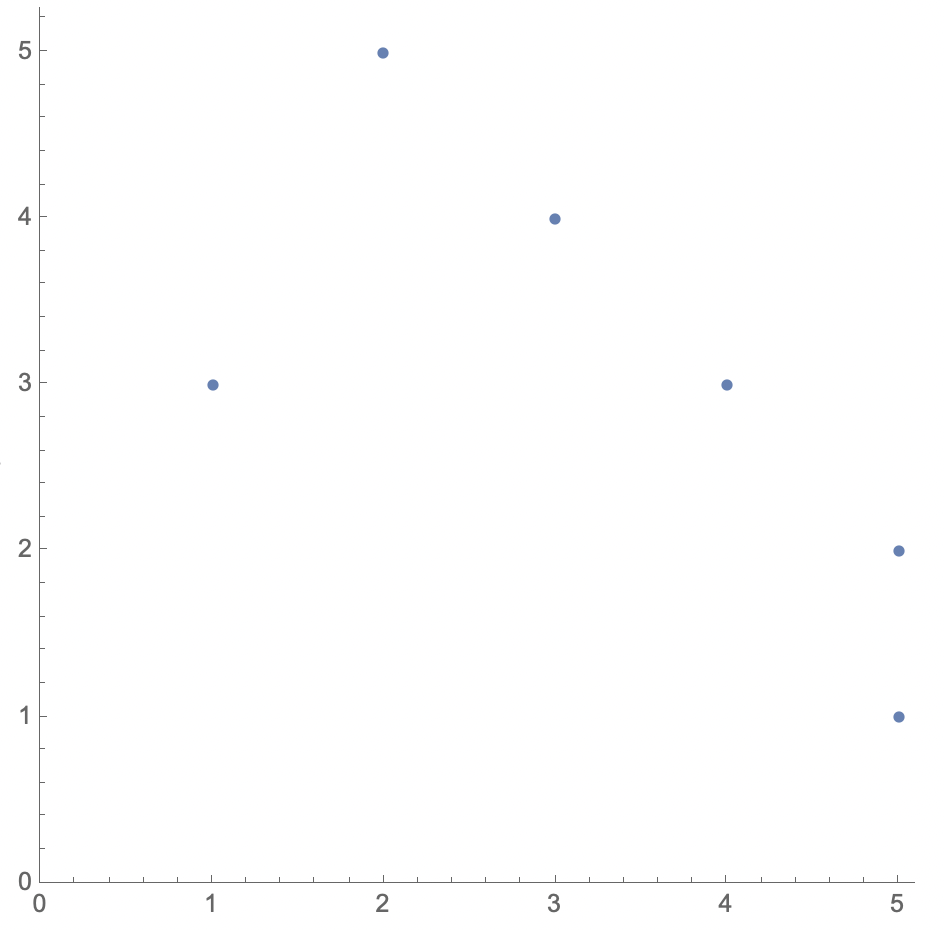
\includegraphics[width=0.6\linewidth]{prob1_scatter.png}
		\caption{Scatter plot with original data points.} % caption of the figure
		\label{fig:fig1}  % Label the figure so you can refer to it in text.
	\end{figure}
	\begin{figure}[H] % This is how figure are placed into latex document
		\centering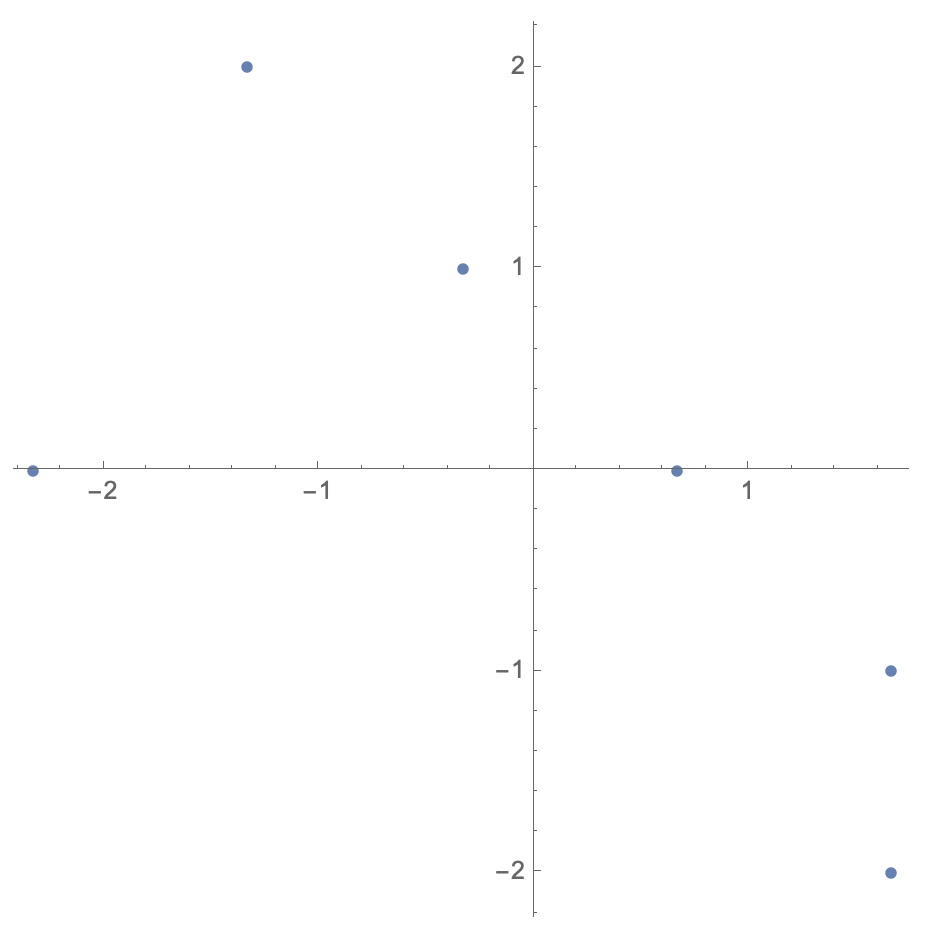
\includegraphics[width=0.6\linewidth]{prob1_scattercent.png}
		\caption{Scatter plot with centered data points.} % caption of the figure
		\label{fig:fig2}  % Label the figure so you can refer to it in text.
	\end{figure}
	Codes (Mathematica):
	\begin{verbatim}
		X = {{1, 3}, {2, 5}, {3, 4}, {4, 3}, {5, 2}, {5, 1}}
		ListPlot[X, PlotRange -> {{0, Automatic}, {0, Automatic}}, 
		AspectRatio -> 1]
		Xcent = # - Mean[X] & /@ X
		ListPlot[Xcent, PlotRange -> {{0, Automatic}, {0, Automatic}}, 
		AspectRatio -> 1]
	\end{verbatim} \\ \\

	\item Now if we want to reduce the dimension from 2 to 1 by PCA, please determine the projection line which crosses the origin (please plot the line based on the scatter-plot figure above).\\ \\
	Since the data points $\mX={{1, 3}, {2, 5}, {3, 4}, {4, 3}, {5, 2}, {5, 1}}$ is not a square matrix, we will perform PCA by ${\vu, \vs, \vv}=SVD(\mX^T\mX)$, and then obtain the loadings of the first principal component by taking the first column of $\vu$. The data points and the projection line obtained with PCA are shown in Fig. 3.\\ \\
	\begin{figure}[H] % This is how figure are placed into latex document
		\centering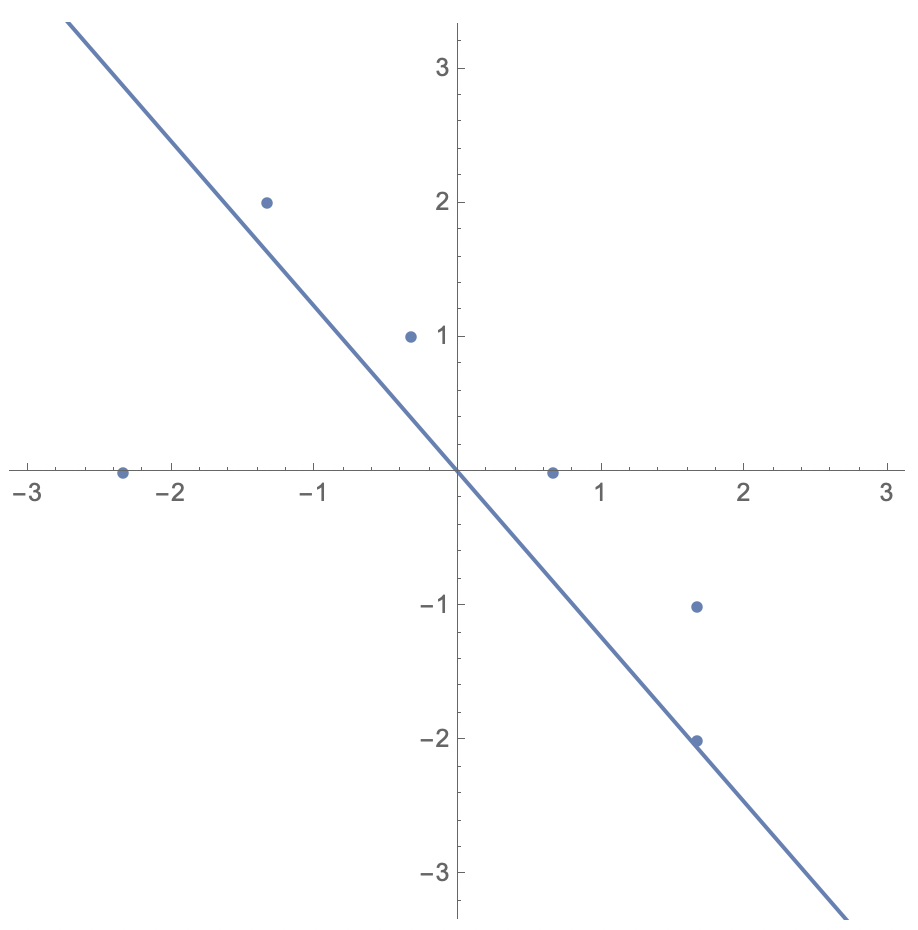
\includegraphics[width=0.6\linewidth]{prob1_pca.png}
		\caption{Scatter plot of data points and projection line obtained with PCA.} % caption of the figure
		\label{fig:fig3}  % Label the figure so you can refer to it in text.
	\end{figure}
	Codes (Mathematica):
	\begin{verbatim}
		{u, s, v} = N@SingularValueDecomposition[Transpose[X].X]
		Show[Plot[u[[1, 1]]/u[[2, 1]] x, {x, 0, 5}], ListPlot[X], 
		PlotRange -> {{0, Automatic}, {0, Automatic}}, AspectRatio -> 1]
	\end{verbatim} \\ \\
	
	\item Assume the first 4 data points belong to one class, while the rest 2 belong to the other. Now if we want to reduce the dimension from 2 to 1 by LDA, please determine the projection line which crosses the origin (you are expected to plot the line based on the scatter-plot figure).\\ \\
	The directional vector of the projection line in LDA is given by: $\vw=\mS^{-1}(\vmu_0-\vmu_1)$, where $\mS_w=\sum_{x\in\mX_0}(\vx-\vmu_0)(\vx-\vmu_0)^T + \sum_{x\in\mX_1}(\vx-\vmu_1)(\vx-\vmu_1)^T$, for the case with two classes $\mX_0$ and $\mX_1$. LDA is performed on the data points aftering centering at the origin. The projection line and the centered data points are shown in Fig. 4.
	\begin{figure}[H] % This is how figure are placed into latex document
		\centering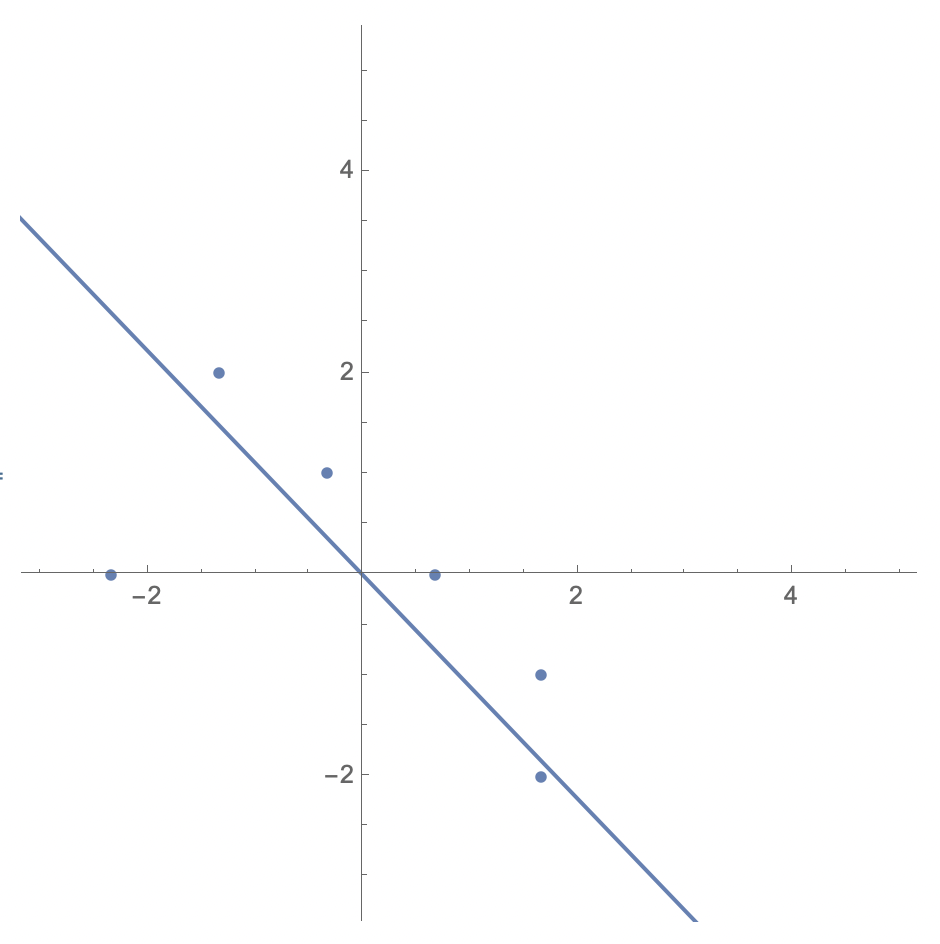
\includegraphics[width=0.6\linewidth]{prob1_lda.png}
		\caption{Scatter plot of data points and projection line obtained with LDA.} % caption of the figure
		\label{fig:fig4}  % Label the figure so you can refer to it in text.
	\end{figure}
\end{enumerate}

\begin{verbatim}
	X1 = Xcent[[1 ;; 4]]
	X2 = Xcent[[5 ;; 6]]
	m1 = Mean[X1]; m2 = Mean[X2];
	m1 = Mean[X1]; m2 = Mean[X2];
	Sw = Plus @@ ((# - m1).Transpose[{# - m1}] & /@ X1) + 
	Plus @@ ((# - m2).Transpose[{# - m2}] & /@ X2);
	w = 1/N @@ Sw*(m1 - m2)
	Show[Plot[w[[1]]/w[[2]] x, {x, -5, 5}], ListPlot[Xcent], 
	PlotRange -> {{-3, 5}, {-3, 5}}, AspectRatio -> 1]
\end{verbatim} \\ \\



\section*{Problem 2}
Given positive data-set $\{\{1,1\},\{2,2\},\{2,3\}\}$, as well as negative data-set $\{\{3,2\},\{3,3\},\{4,4\}\}$, please determine the decision boundary when leveraging $k$-NN where $k=1$ and $k=3$ respectively.\\ \\
To determine the decision boundary, we can generate dense and evenly distributed grids in the 2D plain and classify them with k-NN method. The boundary between different classes of these densely distributed points then indicates the decision boundary of k-NN.\\
The k-NN method is implemented with the\textbf{Classify} function in Mathematica with the specification of classification method: \textbf{Method -> "NearestNeighbors"}. The points in different classes are colored in red and blue respectively, and the boundary between the red and blue regions indicates the decision boundary.\\
\begin{figure}[H] % This is how figure are placed into latex document
	\centering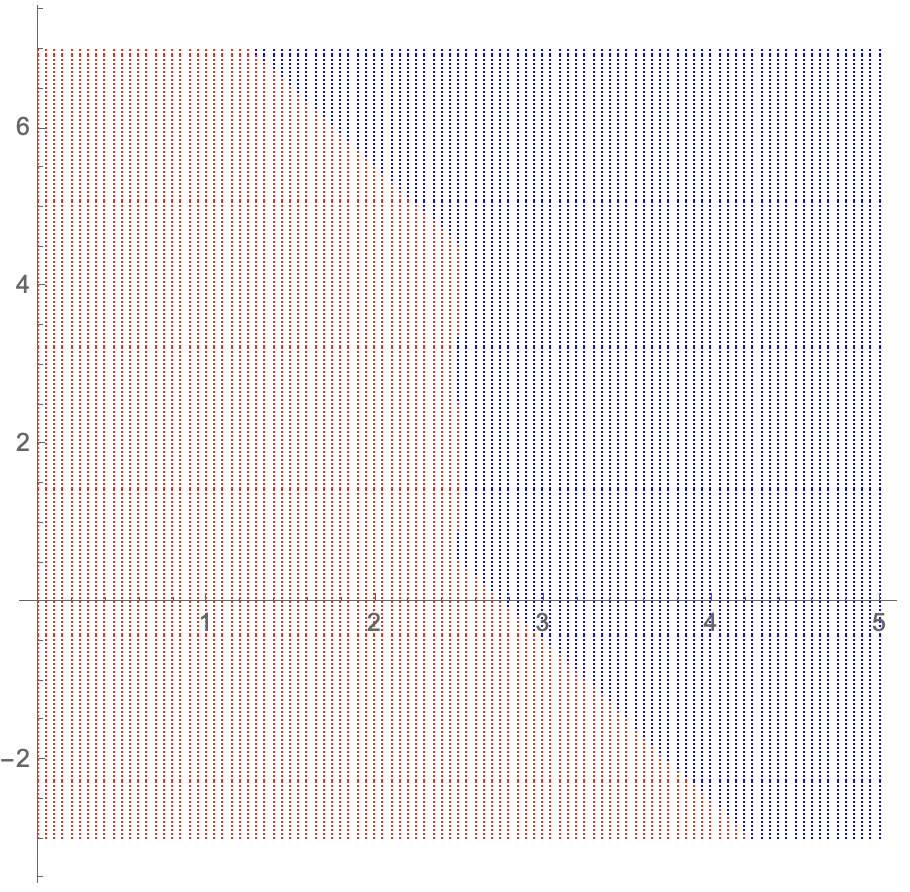
\includegraphics[width=0.4\linewidth]{prob2_k=1.png}
	\caption{Decision boundary of k-NN when k=1.} % caption of the figure
	\label{fig:fig5}  % Label the figure so you can refer to it in text.
\end{figure}
\begin{figure}[H] % This is how figure are placed into latex document
	\centering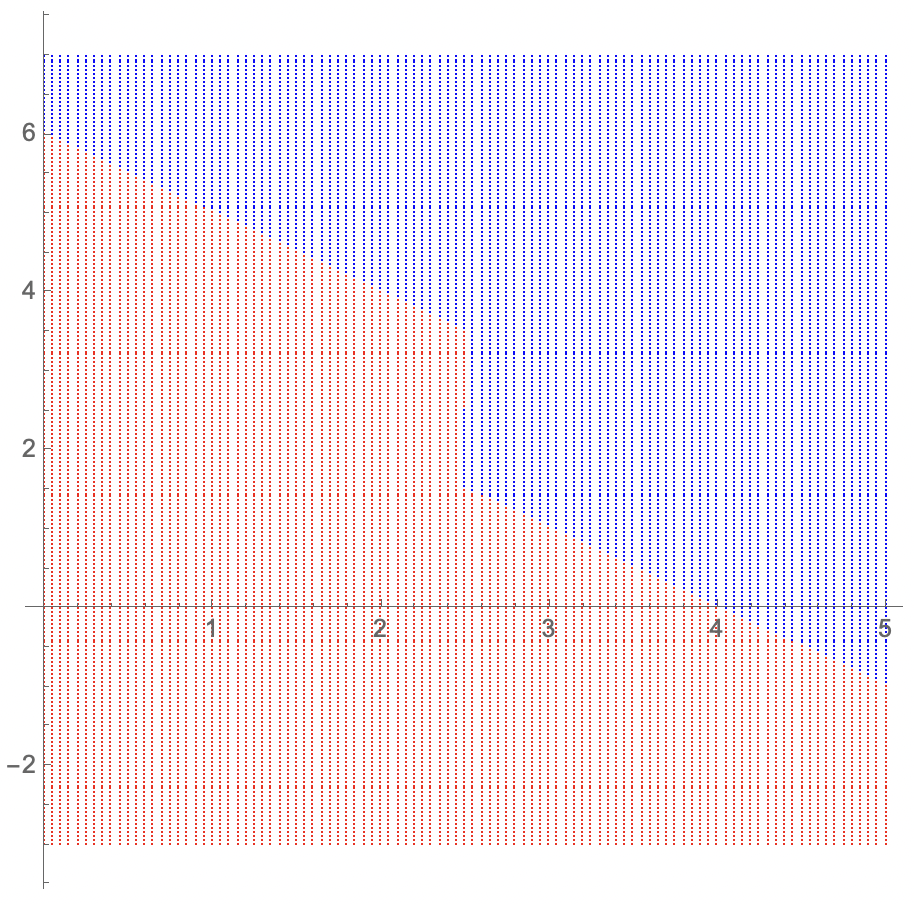
\includegraphics[width=0.4\linewidth]{prob2_k=3.png}
	\caption{Decision boundary of k-NN when k=3.} % caption of the figure
	\label{fig:fig6}  % Label the figure so you can refer to it in text.
\end{figure}
With the increase of $k$ from 1 to 3, we can see that the decision boundary is shifted closer to the positive and negative data sets when the boundaries are far away from these data sets.\\ \\
\textbf{Note: }Ideally, the decision boundary would be completely straight and smooth at $x=2.5$. However we may observe some inflections in the results shown in Figs. 5 and 6. This is mainly due to the insufficient density of the testing data points due to the limited computational power of my personal laptop.\\ \\
\textbf{Codes (Mathematica): }
\begin{verbatim}
	(*k=1*)
	(*Generate testing data points*)
	test = Flatten[
	Table[{i, j}, {i, Range[0, 5, 0.05]}, {j, Range[-3, 7, 0.05]}], 
	1];
	(*Nearest neighbor classifier with k=1*)
	classifier = 
	Classify[Join[# -> 1 & /@ C1, # -> 2 & /@ C2], 
	Method -> {"NearestNeighbors", "NeighborsNumber" -> 1}];
	clustering = AssociationThread[test, classifier[test]];
	ListPlot[ParallelTable[
	Style[x, If[clustering[x] == 1, Red, 
	If[clustering[x] == 2, Blue]]], {x, test}], AspectRatio -> 1]
	
	(*k=3*)
	(*Generate testing data points*)
	test = Flatten[
	Table[{i, j}, {i, Range[0, 5, 0.05]}, {j, Range[-3, 7, 0.05]}], 
	1];
	(*Nearest neighbor classifier with k=3*)
	classifier = 
	Classify[Join[# -> 1 & /@ C1, # -> 2 & /@ C2], 
	Method -> {"NearestNeighbors", "NeighborsNumber" -> 1}];
	clustering = AssociationThread[test, classifier[test]];
	ListPlot[ParallelTable[
	Style[x, If[clustering[x] == 1, Red, 
	If[clustering[x] == 2, Blue]]], {x, test}], AspectRatio -> 1]
\end{verbatim}

\section*{Problem 3}
Given $X, Y, Z$, now please follow the idea/method used in LDA/PCA to find the best solution to:
\begin{equation}
\begin{aligned}
&\underbrace{arg\;max}_{a,b}\;\;{a^TZb}\\
s.t. \ \ &a^TXa =1,\; b^TYb =1
\end{aligned}
\end{equation}
$X$, $Y$ and $Z$ are all symmetric SPD. \\ \\

The objective $\underbrace{arg\;max}_{a,b}\;\;{a^TZb}$ is equivalent to $\underbrace{arg\;min}_{a,b}\;\;{-a^TZb}$. Using two Lagrangian multipliers, $\lambda_1$ and $\lambda_2$ for the two constraints $a^TXa =1$ and $b^TYb =1$, respectively, we can reformulate the objective:
\begin{equation}
	\begin{aligned}
	\underbrace{arg\;min}_{a,b}\;\;{-a^TZb+\lambda_1(a^TXa-1)+\lambda_2(b^TYb-1)}=\underbrace{arg\;min}_{a,b}\;\;{J}
	\end{aligned}
\end{equation}, where $J=-a^TZb+\lambda_1(a^TXa-1)+\lambda_2(b^TYb-1)$ is the objective function.
Taking the derivative of $J$ w.r.t. $a$ and $b$, we get:
\begin{equation}
	\begin{aligned}
		\frac{\partial{J}}{\partial{a}} &= -b^TZ^T+\lambda_1a^T(X+X^T) \\
		&=-b^TZ^T+2\lambda_1a^TX \\
		&= 0
	\end{aligned}
\end{equation}
\begin{equation}
	\begin{aligned}
		\frac{\partial{J}}{\partial{b}} &= -a^TZ+\lambda_2b^T(Y+Y^T) \\
		&=-a^TZ+2\lambda_2b^TY\\
		&= 0
	\end{aligned}
\end{equation}
Right-mutiply $a$ on both sides of Eqn. (3) and $b$ on both sides of Eqn. (4), we have:
\begin{equation}
	\begin{aligned}
		b^TZ^Ta&=b^TZa\\
		&=2\lambda_1
	\end{aligned}
\end{equation}
and 
\begin{equation}
	\begin{aligned}
		a^TZ^Tb=2\lambda_2
	\end{aligned}
\end{equation}
From Eqns. (5) and (6), we know that $\lambda_1=\lambda_2=\lambda$. To maximize $a^TZ^Tb$ is equivalent to maximizing $\lambda$.

Take the transpose of Eqns. (3) and (4): 
\begin{equation}
	\begin{aligned}
		Zb-2\lambda Xa=0
	\end{aligned}
\end{equation}
and 
\begin{equation}
	\begin{aligned}
		Za-2\lambda Yb=0
	\end{aligned}
\end{equation}

Then left-multiply $X^{-1}$ on both sides of Eqn. (7) and $Y^{-1}$ on Eqn. (8), we have:
\begin{equation}
	\begin{aligned}
		X^{-1}Zb=2\lambda a, \\
		a=\frac{X^{-1}Zb}{2\lambda}
	\end{aligned}
\end{equation}
and 
\begin{equation}
	\begin{aligned}
		Y^{-1}Za=2\lambda b, \\
		b=\frac{Y^{-1}Za}{2\lambda }
	\end{aligned}
\end{equation}
Combining Eqns. (9) and (10):
\begin{equation}
\begin{aligned}
	&Y^{-1}Za=Y^{-1}Z\frac{X^{-1}Zb}{2\lambda}=2\lambda b, \\
	&Y^{-1}ZX^{-1}Zb=4\lambda^2b
\end{aligned}
\end{equation}
\begin{equation}
	\begin{aligned}
		&X^{-1}Zb=x^{-1}Z\frac{Y^{-1}Za}{2\lambda}=2\lambda a, \\
		&X^{-1}ZY^{-1}Za=4\lambda^2a
	\end{aligned}
\end{equation}
Eqns (11) and (12) are eigenvlue decomposition problems $Aa=4\lambda^2a$ and $Bb=4\lambda^2b$, where $A=X^{-1}ZY^{-1}Z$ and $B=Y^{-1}ZX^{-1}Z$.
The eigenvalue decomposition is cummulative w.r.t. matrix multiplication, i.e. the eigenvalues and eigenvectors of $(MN)v=\sigma v$ is the same as $(MN)v=\sigma v$. Note that if we define $M=X^{-1}Z$ and $N=Y^{-1}Z^T$, then $A=MN$, $B=NM$, and therefore $A$ and $B$ have the same set of eigenvalues $\{\sigma_i\}$, where $\sigma=4\lambda^2$. The corresponding eigenvectors $\{u_i\}$ for $A$ $\{v_i\}$ for $B$ ($i=1,2,...,n$) are parrallel to each other, which are sorted in decreasing order of $\sigma_i$. To maximize $(a^TZb)^T$, or equivalently $\lambda^2$, we can set:
\begin{equation}
	\begin{aligned}
		&a=u_1\\
		&b=v_1
	\end{aligned}
\end{equation}\\ \\

\textbf{Alternative method:}\\
From the constraints, we have
\begin{equation}
	\begin{aligned}
		&a^TXa=a^TX^{1/2}X^{1/2}a\\
		&b^TYb=b^TY^{1/2}Y^{1/2}b
	\end{aligned}
\end{equation}
Define $u^Tu=1$, $v^Tv=1$, and plug back into the objective function $J=a^TZb$, we have: $J==u^TX^{-1/2}ZY^{-1/2}v$. If we perform $SVD(X^{-1/2}ZY^{-1/2})=[U,S,V]$, to maximize $J=a^TZb$ we can take $u=U(:,1)$, $v=V(:,1)$.
 

%Since $a^TXa=a^TX^Ta=1$, by right-multiplation of $a$ on both sides of eqn. (3), we get:
%\begin{equation}
%	\begin{aligned}
%		&-b^TZ^Ta+\lambda_1a^T(X+X^T)a=0\\
%		&b^TZ^Ta=(a^TZb)^T=2\lambda_1
%	\end{aligned}
%\end{equation}
%By right-multiplation of $b$ on both sides of eqn. (4), we get:
%\begin{equation}
%	\begin{aligned}
%		&-a^TZb+\lambda_2b^T(Y+Y^T)b=0\\
%		&a^TZb=2\lambda_2
%	\end{aligned}
%\end{equation}
%Combining Eqn. (5) and (6), we have: $(a^TZb)^Ta^TZb=4\lambda_1\lambda_2$, which means that to maximize $a^TZb$ is equivalent to maximizing $\lambda_1\lambda_2$.
%Take the transpose on both sides of Eqn. (3) and (4), we get: 
%\begin{equation}
%	\begin{aligned}
%		&Zb=\lambda_1(X+X^T)a\\
%		&b=\lambda_1Z^{-1}(X+X^T)a
%	\end{aligned}
%\end{equation}
%and 
%\begin{equation}
%	\begin{aligned}
%		&Z^Ta=\lambda_2(Y+Y^T)b
%		&a=\lambda_2(Z^T)^{-1}(Y+Y^T)b
%	\end{aligned}
%\end{equation}
%
%
%Plug Eqn. (7) into Eqn. (8), we get:
%\begin{equation}
%	\begin{aligned}
%		&Z^Ta=\lambda_1\lambda_2(Y+Y^T)Z^{-1}(X+X^T)a\\
%		&[(X+X^T)^{-1}Z(Y+Y^T)^{-1}Z^T]a=\lambda_1\lambda_2a
%	\end{aligned}
%\end{equation}
%Define $A=(X+X^T)^{-1}Z(Y+Y^T)^{-1}Z^T$, and Eqn. (9) can be seen as an eigenvalue problem:
%\begin{equation}
%	\begin{aligned}
%		&Aa=\lambda_1\lambda_2a
%	\end{aligned}
%\end{equation}
%Similarly, plug Eqn. (8) into (7), we can get:
%\begin{equation}
%	\begin{aligned}
%		[(Y+Y^T)^{-1}Z^T(X+X^T)^{-1}Z]b=\lambda_1\lambda_2b
%	\end{aligned}
%\end{equation}
%Define $B=(Y+Y^T)^{-1}Z^T(X+X^T)^{-1}Z$, we can similarly obtain:
%\begin{equation}
%	\begin{aligned}
%		Bb=\lambda_1\lambda_2b
%	\end{aligned}
%\end{equation}
%The eigenvalue decomposition is cummulative w.r.t. matrix multiplication, i.e. the eigenvalues and eigenvectors of $(MN)v=\sigma v$ is the same as $(MN)v=\sigma v$. Note that if we define $M=(X+X^T)^{-1}Z$ and $N=(Y+Y^T)^{-1}Z^T$, then $A=MN$, $B=NM$, and therefore $A$ and $B$ have the same set of eigenvalues $\{\sigma_i\}$ and corresponding eigenvectors $\{v_i\}$ ($i=1,2,...,n$), which are sorted in decreasing order of $\sigma_i$. To maximize $(a^TZb)^T$, or equivalently $\lambda_1\lambda_2$, we can set:
%\begin{equation}
%	\begin{aligned}
%		a=b=v_1
%	\end{aligned}
%\end{equation}
%, which is the eigenvector of $A$ and $B$ corresponding to the largest eigenvalue $\lambda_1\lambda_2=\sigma_1$.
%To obtain the $a$ that maximizes $\lambda_1\lambda_2$, we can perform $SVD(A)=[U_a,S_a,V_a]$, where $A=Z^T(X+X^T)^{-1}Z(Y+Y^T)^{-1}$. The $i$-th column $u_{ai}$ of $U_a$ is the eigenvector of $A$ with the corresponding eigenvalue $s_{ai}$, which is the $i$-th singular value given by diagonal elements of $S$ in decreasing order. In this case, by comparing the SVD formulation with the eigenvalue problem in Eqn. (10) we have $\lambda_1\lambda_2=s_i$. So to maximize  $\lambda_1\lambda_2$, we can make 
%\begin{equation}
%	\begin{aligned}
%		&a=u_{a1}\\ 
%		&\lambda_1\lambda_2=s_{a1}
%	\end{aligned}
%\end{equation}
%Similarly, we can have:
%\begin{equation}
%	\begin{aligned}
%		&b=u_{b1}\\ 
%		&\lambda_1\lambda_2=s_{b1}
%	\end{aligned}
%\end{equation}
%, where $B=Z(Y+Y^T)^{-1}Z^T(X+X^T)^{-1}$, $SVD(A)=[U_b,S_b,V_b]$, $u_{b1}$ is the first column of $U_b$ and $s_{b1}$ is the first singular value of $B$.


\end{document}
